\documentclass[12pt]{article}
\usepackage{amsmath, amssymb, amsthm, graphicx, epsfig, fancyhdr, graphicx, amsfonts}
\usepackage{algorithm}
\usepackage[noend]{algpseudocode}
\usepackage[utf8]{inputenc}

\title{Math 240 Overleaf Form} 
\author {Laouen belloli}

\setlength{\headheight}{28pt}
\pagestyle{fancy}
\fancyhf{}
\fancyhead[R]{Laouen Belloli \\ Automatic creation of Metabolic Network in PDEVS}
\fancyfoot[C]{\thepage}


\begin{document}

\section*{summary of the reading}
After spend 3 days reading both books,''Principles of Biochimistry`` from Lehninger and ''Chemistry \& Chemical Reactions``  from Kotz \& Treichel, I restart with another diferent aprouch to the problem.

Since we only want to consider reaction leaded by enzymes, I don't see why to model the reactions instead of model the cell components. A cell have many components and fenomens, but we can only model these components and fenomens needed. In this way, in the future, we can add others components or fenomens as we'll need it.

\section*{Boost CD++}
Boost C++ is Damian's tool to model and run simulation of Parallel DEVS. This formalism has not (in/out)-ports and a filter must be defined for all models in order to ignore the message that are not directed to them.

\subsection*{the Filter model}
Since BCDPP (Boost CD++) has no ports, all models needs a filter to ignore the messages that are not directed to the them.
The next DEVS-graph explain the behavior of the filter atomic model.


\begin{figure}[h!]
 \centering
  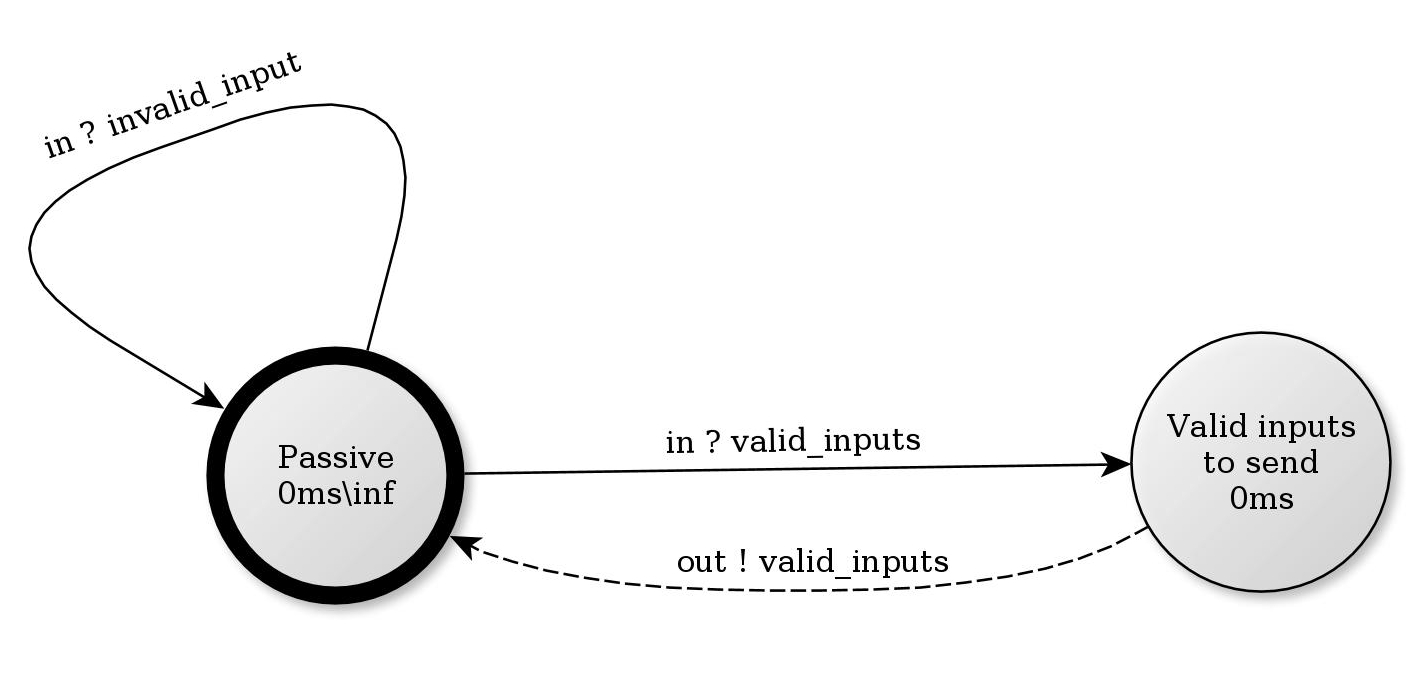
\includegraphics[width=350px]{atomic-filter.jpg}
 \caption{Filter atomic model.}
\end{figure}

\newpage
\section*{New aprouch to the cell model}  
A cell have basicly three components that matter for us, a membrane (where transportation reactions happens), a cytoplasm (where some reaction happens) and organelles (different compartments with their own reactions).
There is a lot of other components but I am not considering them.
all this components have enzymes and therefore reaction happens there. the membrane is who take care of the communication between the outside and the cytoplasm, this communication is leaded by enzymes by making transportation reactions. The cytoplasm can do reactions and pass his molecules to the organelles and membrane, and the same happens with the organelle how can do reactions and give back products to the cytoplasm.

my Idea now is to model the next components: the enzymes, the organelles, the cytoplasm, the membrane and the space like a discrete tridimensional space in $\mathbb{Z}^3$. Then join all these models in a coupled model of a cell. The molecules are the input and output, and they are only in the messages and states.

\subsection*{generic and instance models (implementation of automatic modeling)}
All the models in Boost CD++ are defined as c++ classes. The idea is to design generic models of these component as c++ classes, and then dynamically create the different instances, so for example, the generic class enzyme will have an empty list of reactants as a property of his class, but when a particular instance of enzyme model is created, it will use the list of reactant passed as parameter to the class constructor to set the reactants of this particular enzyme model.

\newpage
\section*{the models}

\subsection*{the enzyme}
The coupled model for an enzyme is the next:

\begin{figure}[h!]
 \centering
  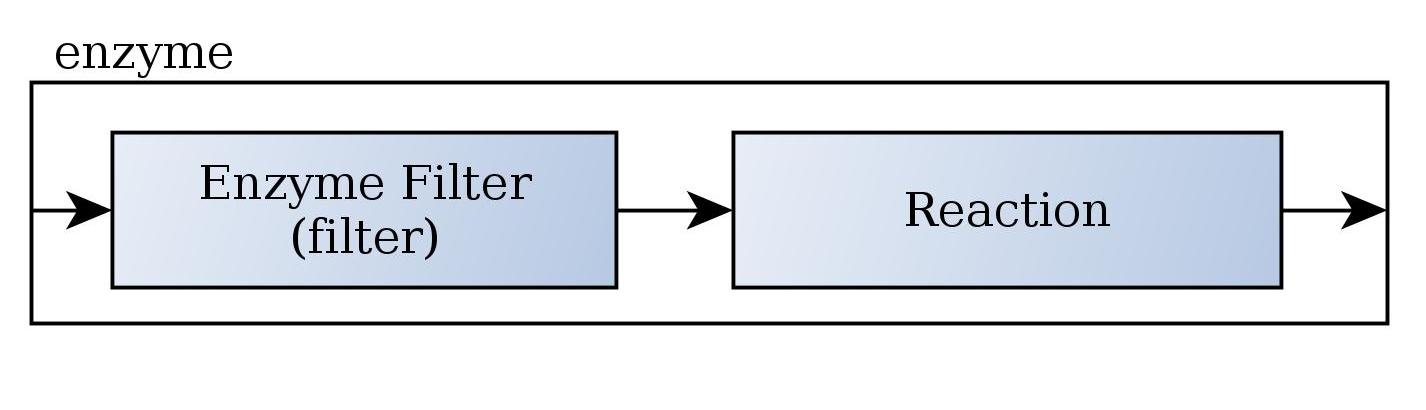
\includegraphics[width=1\textwidth]{coupled-enzyme.jpg}
 \caption{enzyme coupled model: blue color mean atomic models. The reaction and filter models are generic classes, then the coupled model shown a generic class for a coupled enzyme model. To create a particular instance of the enzyme model we need first, create particular instances of a reaction and a filter model.}
\end{figure}

The reaction model, is a generic model who is in charge to bind the reactants/substrates and when all necessaries substrates are in the enzyme, the reaction start.
In every discrete interval of time (constant intervals), the reaction can lose one or more substrates that was bound to the enzyme, a random function with the appropriate distribution can decide in every interval of time which substrate will stay longer and which not. If a reaction is reversible and there is both substrates and products bound to the enzyme, the reaction cannot start until one of them (substrates or products) is gone.

moreover an enzyme represent a single unit who can catalyze only one unit of reactants, producing only one unit of products. 

Also, Two enzyme cannot be in the same space, but probably, two enzyme of a same kind are attracted to stay close each other.

\newpage
The next DEVS-graph represent the behavior of a reaction atomic model.

\begin{figure}[h!]
 \centering
  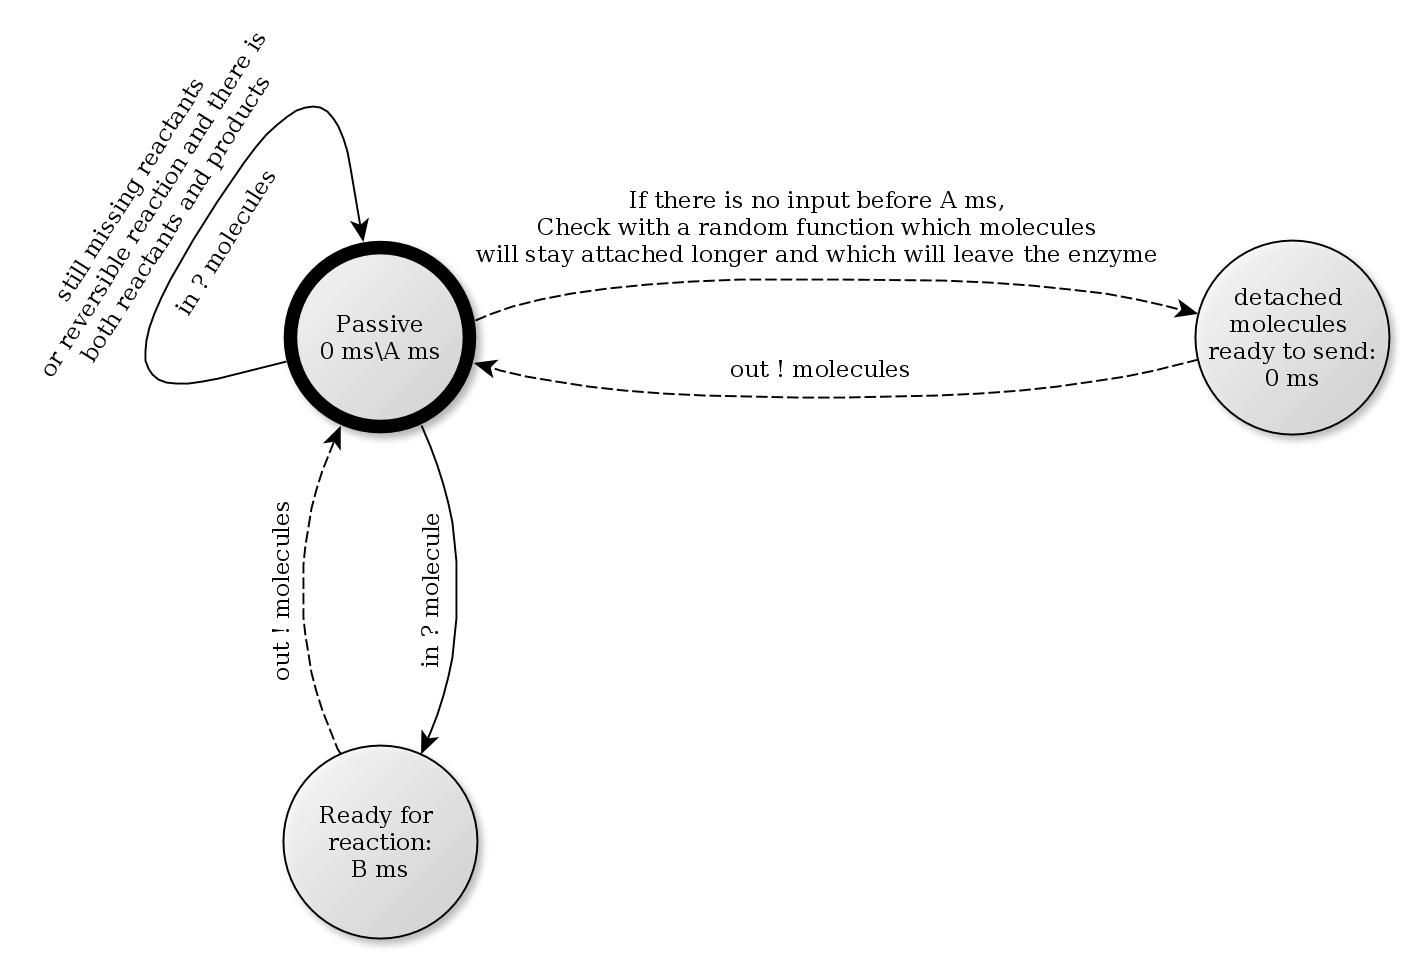
\includegraphics[width=1\textwidth]{atomic-reaction.jpg}
 \caption{DEVS-graph of a Reaction atomic model.}
\end{figure}

\newpage
\subsection*{the organelle}

The coupled model for an organelle is the next:

\begin{figure}[h!]
 \centering
  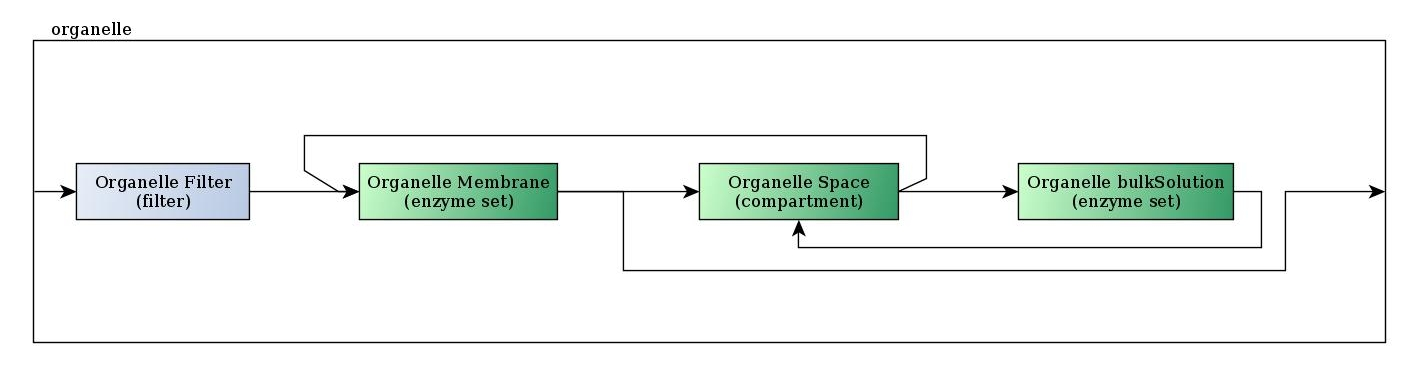
\includegraphics[width=400px]{coupled-organelle.jpg}
 \caption{organelle coupled model: blue color mean atomic models, green color mean coupled model. The models of the enzyme set, the filter and the compartment are generic classes, then the coupled model shown a generic class for a coupled organelle model. To create a particular instance of the organelle model, we need first, create particular instances of a enzyme set, compartment and filter model.}
\end{figure}

the coupled models enzyme set and compartment will be explained in the next subsections. but just to understand the organelle model, here is a short explanation.

\subsubsection*{the enzyme set}
this model has a list of enzymes and when a molecule arrive to the input, it will be directed to the correct enzyme, this enzyme can do his functions and depending on if a reaction has being triggered or not, the output products will be give back by the output of the model.

\subsubsection*{the compartment}
This model is basically a three dimensional space where the enzymes and molecules are moving and when a molecule is in the same place that an enzyme, the model will send the molecule to the enzyme model which correspond with this space.

\subsubsection*{the organelle coupled model}
the molecules arrive to the membrane and after the transportation reaction happens it goes to the compartment where it will be moving until it found an enzyme and then, the compartment model send the molecule to this enzyme in the inner model, after the reaction occur, the inner model give back the output products to the compartment. Some times, moving molecule in the compartment can collapse with the edge of the tridimensional space and collapse with one enzyme in the membrane, in this case, the compartment send the molecule to the enzyme in the membrane and after the transportation reaction, the membrane will put the molecule in the output of the model.

\subsection*{the cytoplasm}
The coupled model for the cytoplasm is the next:

\begin{figure}[h!]
 \centering
  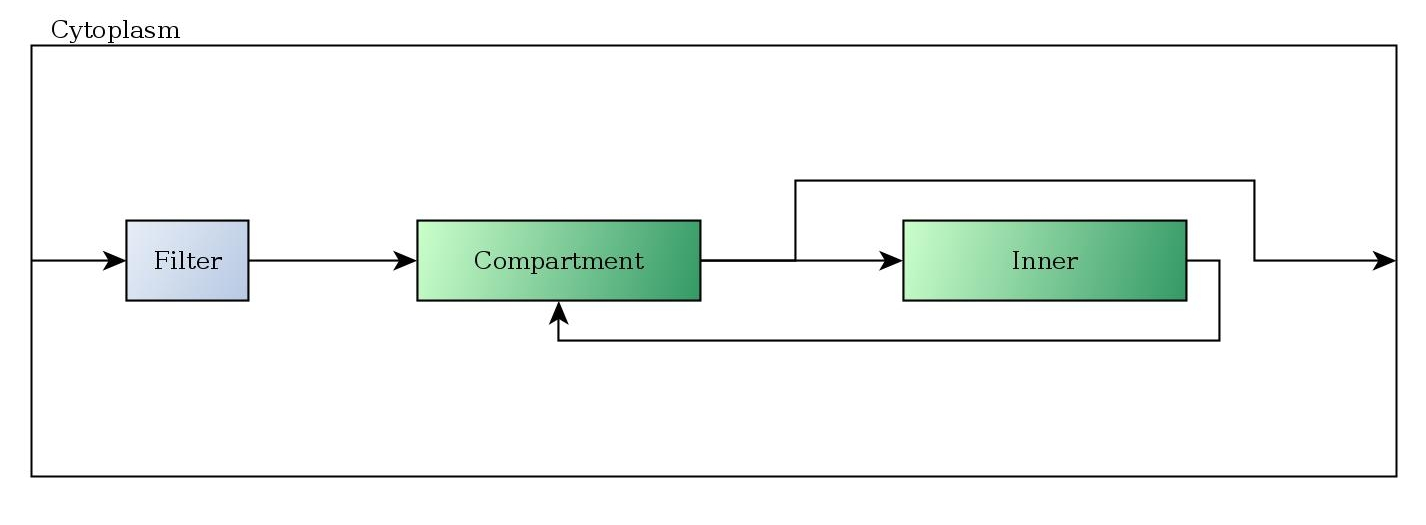
\includegraphics[width=1\textwidth]{coupled-cytoplasm.jpg}
 \caption{cytoplasm coupled model: blue color mean atomic models, green color mean coupled model. The models of the enzyme set, the filter and the compartment are generic classes, then the coupled model shown a generic class for a coupled cytoplasm model. To create a particular instance of the cytoplasm model, we need first, create particular instances of a enzyme set, compartment and filter model}
\end{figure}

The cytoplasm model is similar to an organelle model, with the main difference that the cytoplasm does not have membrane, the membrane who communicate the input molecule with the compartment of the cytoplasm is the cell membrane. So the compartment send the molecule to an external enzyme in the cell membrane or to an enzyme in an organelle membrane.

\newpage
\subsection*{the compartment (space model)}

the coupled model for a compartment is the next:

\begin{figure}[h!]
 \centering
  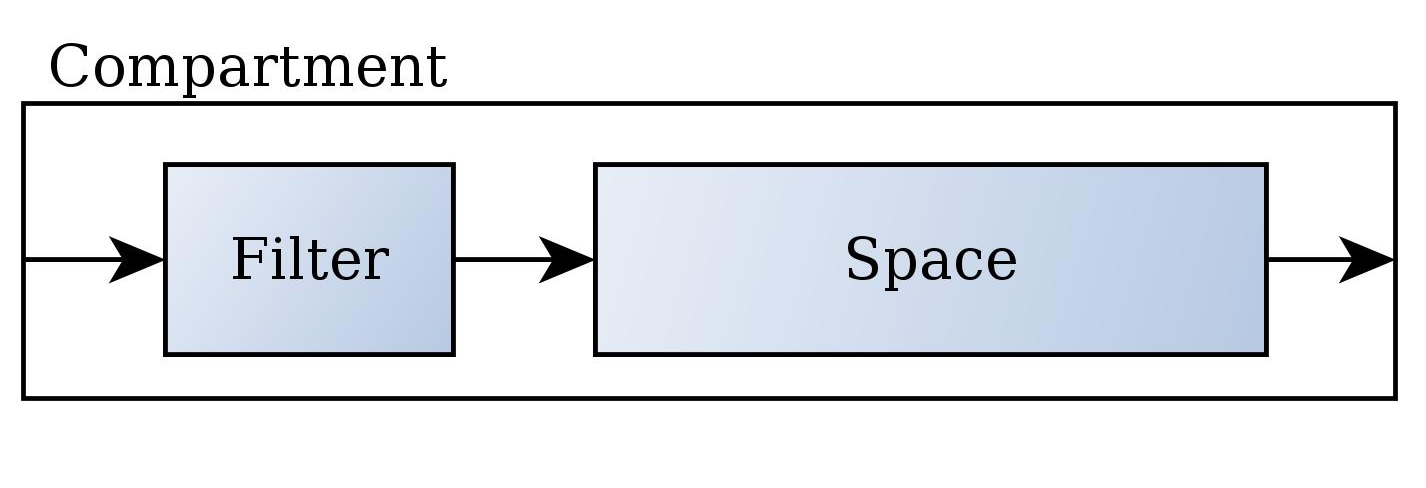
\includegraphics[width=300px]{coupled-compartment.jpg}
 \caption{compartment coupled model: blue color mean atomic models. The space and filter models are generic classes, then the coupled model shown a generic class for a coupled compartment model. To create a particular instance of the compartment model we need first, create particular instances of a space and a filter model.}
\end{figure}

The space is a generic model with a three dimensional set of discrete points, this set of point are the points that belongs to the compartment. each point have the information of the enzymes and/or molecules who are there. When a molecule is in the same space of a enzyme, the model will send this molecule to the remote model of the enzyme who take care of the reaction by the output in a message.
 
The next DEVS-graph represent the behavior of a Space atomic model.


\begin{figure}[h!]
 \centering
  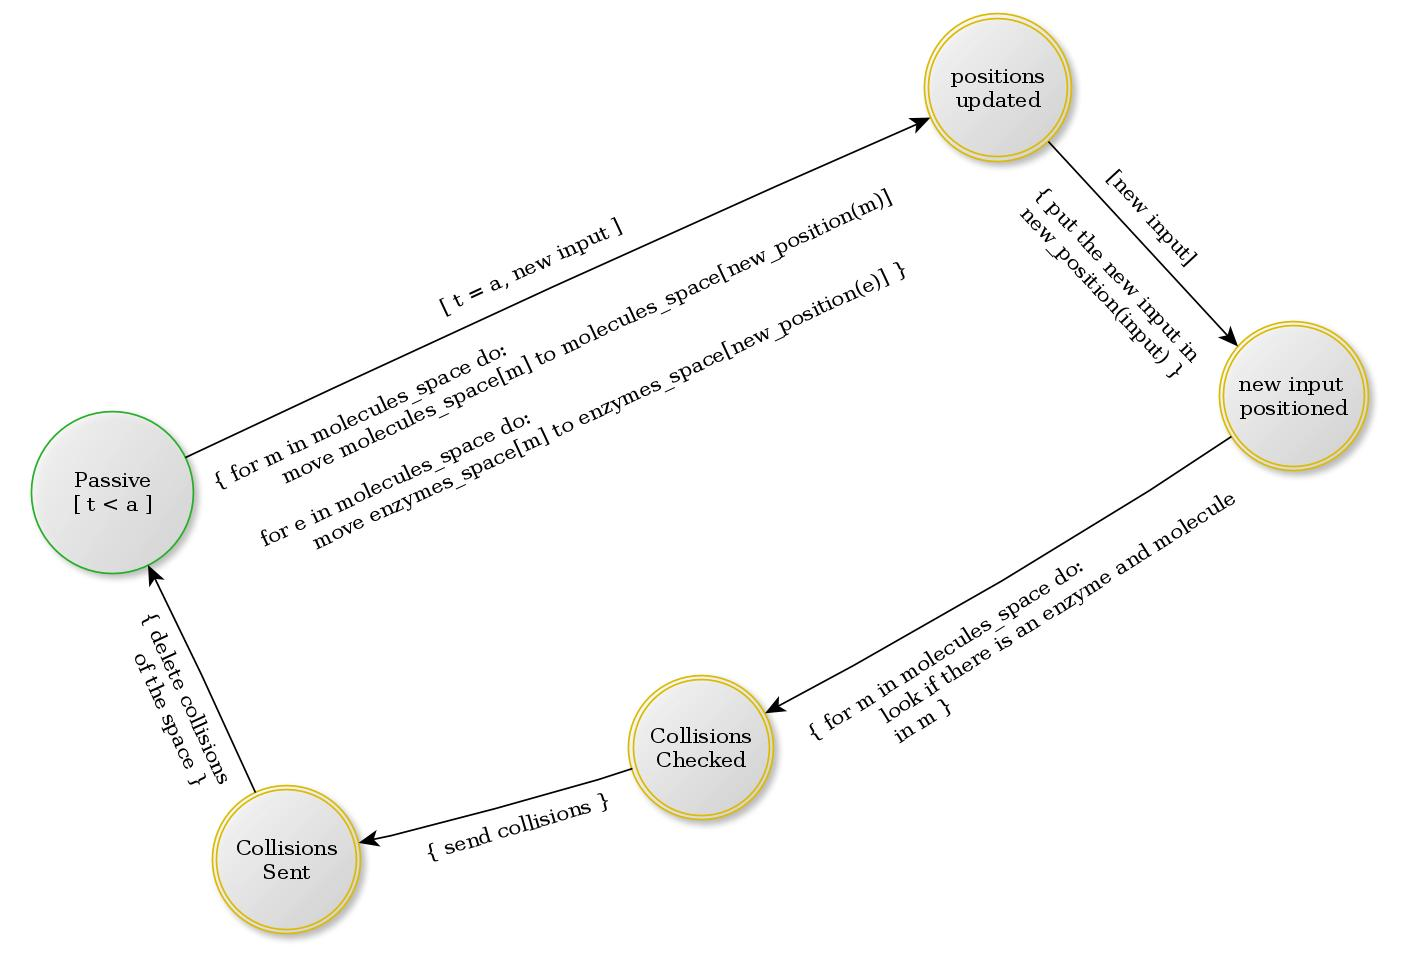
\includegraphics[width=300px]{atomic-space.jpg}
\end{figure}

\newpage
\subsection*{The enzyme set}

The coupled model for an enzyme set is the next:

\begin{figure}[h!]
 \centering
  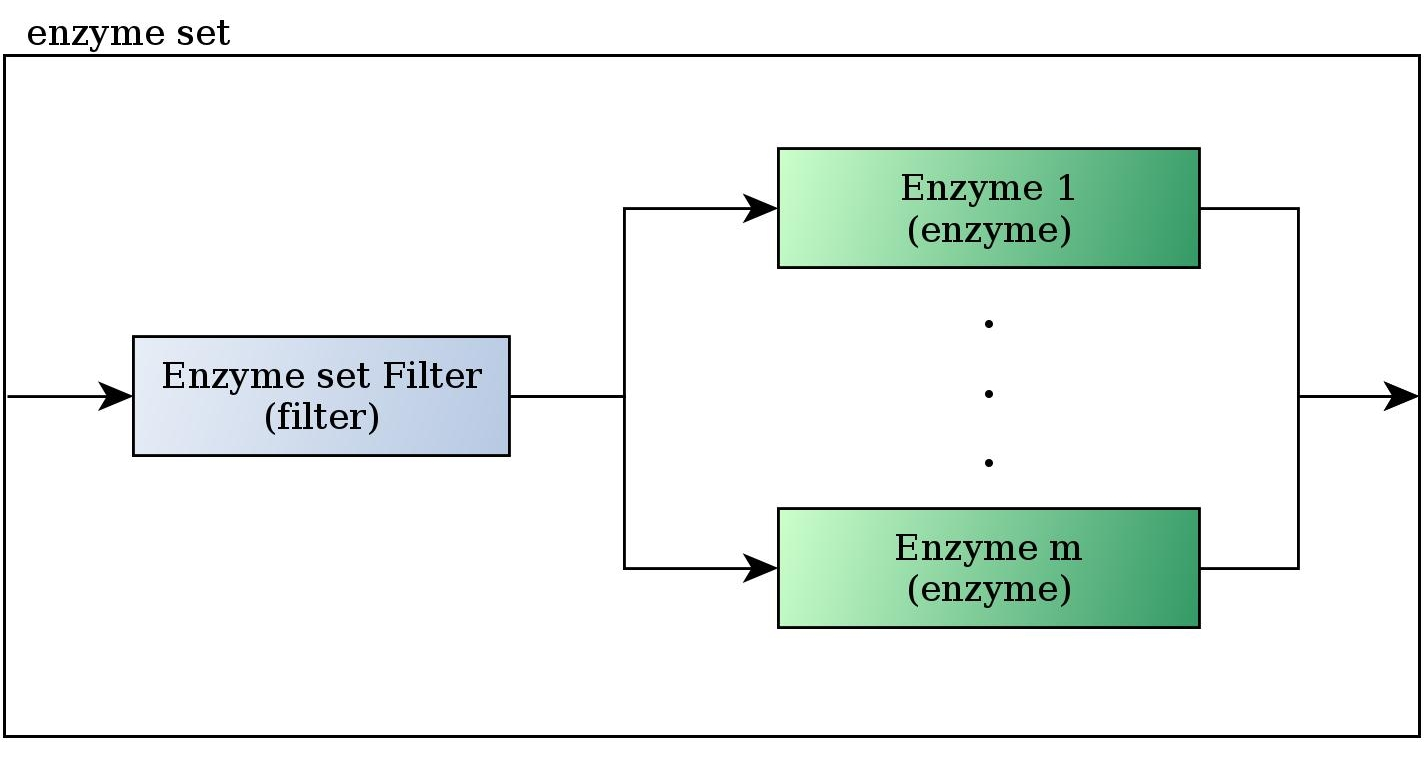
\includegraphics[width=300px]{coupled-enzyme-set.jpg}
 \caption{ensyme set coupled model: blue color mean atomic models, green color mean coupled models. The models of the enzymes and the filter are generic classes, then the coupled model shown a generic class for a coupled enzyme set model. To create a particular instance of the enzyme set model, we need first, create particular instances of the enzymes and a filter model.}
\end{figure}

The model is a list of enzymes, when an input arrive, it will goes to the correct enzyme. The molecules come with the information about which enzyme is the receptor, this information it will be given by the compartment model when it send the molecule to the enzyme set.

\subsection*{the cell model}
Finally once we have all these model, we are able to present the cell model which is a really simple coupled model, but if we expand all the submodels until have only atomic models, it comes bigger. The good thing here, is that there is only 3 atomic models, and as we can see in the DEVS-graphs they are not to complicated.

\newpage
The coupled model for the cell is the next:

\begin{figure}[h!]
 \centering
  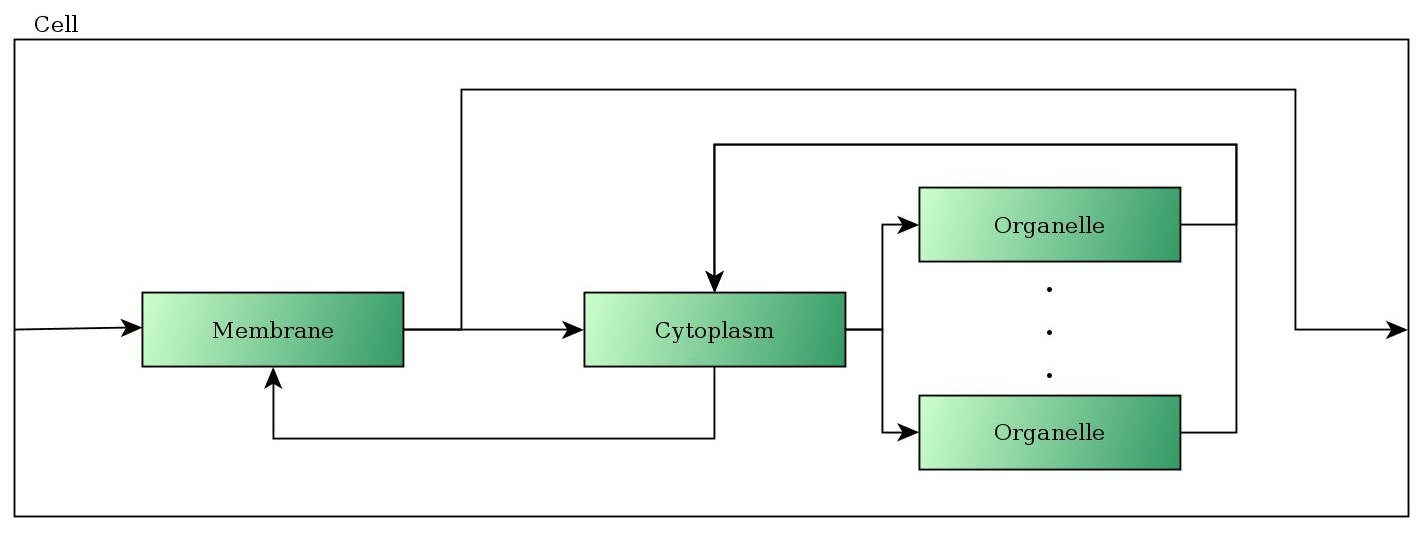
\includegraphics[width=300px]{coupled-cell.jpg}
 \caption{cell coupled model: Green color mean coupled models. The models of the enzyme set, the cytoplasm and the organelles are generic classes, then the coupled model shown a generic class for a coupled cell model. To create a particular instance of the cell model, we need first, create particular instances of the enzyme set, cytoplasm and filter model}
\end{figure}

We can see that a cell is basically what we know about cells in real life, The input is connected to a membrane (the cell membrane) and this membrane give the coming up molecules to the cytoplasm where reaction can happens and some times the cytoplasm pass this molecules to the organelles (this happen when a molecule is in the same place that one enzyme of the organelle membrane) and after be in the organelles and pass through reactions in there, the products of the organelles can go to the Cytoplasm and some times to the membrane and go outside (this happens when the molecules are in the same place that one enzyme of the cell membrane).

\subsection*{conclusions}

The Idea then is to take the information about all the enzyme dynamically from the SBML file and create al the instances of atomic enzymes, filters and spaces models. Then also dynamically through c++ loops create the coupled model with all the connections and thus, the model will be ready to start the simulations.
The most difficult part of this model I think is the space in $\mathbb{Z}^3$ because I think is not specified in the SMBL, but maybe in can be well approximated by some known shape like a ball. I don't know. This is one of the problems that I want to talk in the next meeting. Also I need to talk about the random functions and how the enzymes and substrate are swimming, if they go only in one direction or a random function in the neighborhood said the next position in each interval time, I don't know. I think maybe this part can be modeled with cell-DEVS, but I think that Damian didn't do a Cell-DEVS tools.
Also I have some specific questions about the SBML file.


\end{document}